\documentclass{standalone}
\usepackage{tikz}
\usetikzlibrary{arrows.meta}

\tikzstyle{input-node}=[fill=white,circle,thick,draw]
\tikzstyle{hidden-node}=[fill=white,circle,thick,draw]
\tikzstyle{dropout-node}=[fill=black!20,circle,thick,draw]
\tikzstyle{output-node}=[fill=white,circle,thick,draw]

\tikzstyle{black-line}=[draw=black,very thick]
\tikzstyle{red-line}=[draw=red,very thick]


\begin{document}
    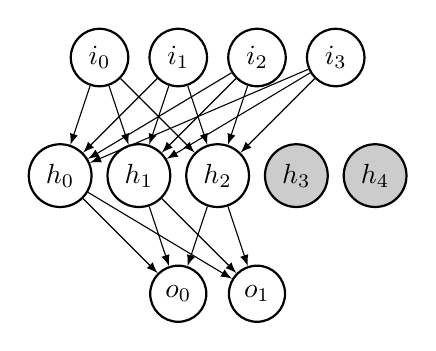
\begin{tikzpicture}
        \begin{scope}
            \node[input-node] at (-1.5,0) (i0) {$i_0$};
    		\node[input-node] at (-0.5,0) (i1) {$i_1$};
    		\node[input-node] at (0.5,0) (i2) {$i_2$};
    		\node[input-node] at (1.5,0) (i3) {$i_3$};			
    		\node[hidden-node] at (-2,-1.5) (h0) {$h_0$};
    		\node[hidden-node] at (-1,-1.5) (h1) {$h_1$};
    		\node[hidden-node] at (0,-1.5) (h2) {$h_2$};
    		\node[dropout-node] at (1,-1.5) (h3) {$h_3$};			
    		\node[dropout-node] at (2,-1.5) (h4) {$h_4$};			
    		\node[output-node] at (-0.5,-3) (o0) {$o_0$};			
    		\node[output-node] at (0.5,-3) (o1) {$o_1$};			
    		
    		\foreach \a in {0, 1, 2, 3}{
    			\foreach \b in {0, 1, 2}
    			\draw[-latex] (i\a) -- (h\b);
    		}
    		\foreach \a in {0, 1, 2}{
    			\foreach \b in {0, 1}
    			\draw[-latex] (h\a) -- (o\b);
    		}
        \end{scope}
    \end{tikzpicture}
\end{document}
